\documentclass{standalone}

\usepackage{tikz}
\usepackage{circuitikz}

\tikzset{block/.style = {draw, fill=white, very thick, rectangle, minimum height=1cm, minimum width=2cm},
         lblock/.style={draw,fill=white,very thick, rectangle, minimum height=3cm, minimum width=1cm},
         sum/.style= {draw, fill=white, very thick, circle, node distance=0.5cm}}

         
\begin{document}
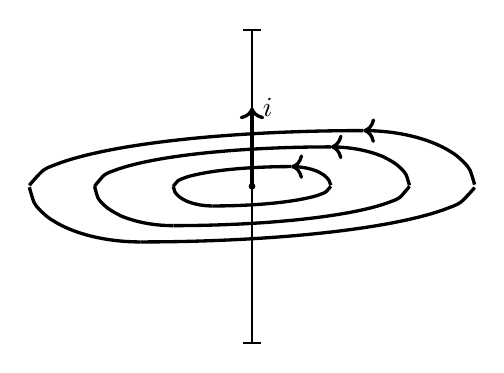
\begin{tikzpicture}[scale=2]
    \draw[<-, very thick]plot[smooth, domain=0.707:1.414](\x,{0.5*(0.5-(\x-0.707)^2)^0.5});
        \draw[-, very thick]plot[smooth, domain=-1.414:-0.707](\x,{-0.5*(0.5-(\x+0.707)^2)^0.5});
        \draw[-, very thick]plot[smooth, domain=-1.414:0.707](\x,{1/6*(4.5-(\x-0.707)^2)^0.5});
        \draw[-, very thick]plot[smooth, domain=-0.707:1.414](\x,{-1/6*(4.5-(\x+0.707)^2)^0.5});

        \draw[<-, very thick]plot[smooth, domain=0.5:1](\x,{0.5*(0.25-(\x-0.5)^2)^0.5});
        \draw[-, very thick]plot[smooth, domain=-1:-0.5](\x,{-0.5*(0.25-(\x+0.5)^2)^0.5});
        \draw[-, very thick]plot[smooth, domain=-1:0.5](\x,{1/6*(2.25-(\x-0.5)^2)^0.5});
        \draw[-, very thick]plot[smooth, domain=-0.5:1](\x,{-1/6*(2.25-(\x+0.5)^2)^0.5});

        \draw[<-, very thick]plot[smooth, domain=0.25:0.5](\x,{0.5*(0.0625-(\x-0.25)^2)^0.5});
        \draw[-, very thick]plot[smooth, domain=-0.5:-0.25](\x,{-0.5*(0.0625-(\x+0.25)^2)^0.5});
        \draw[-, very thick]plot[smooth, domain=-0.5:0.25](\x,{1/6*(0.5625-(\x-0.25)^2)^0.5});
        \draw[-, very thick]plot[smooth, domain=-0.25:0.5](\x,{-1/6*(0.5625-(\x+0.25)^2)^0.5});

        \draw[|-|, thick](0,-1)--(0,1);
        \draw[->, very thick](0,0)--(0,0.5)node[right]{$i$};
        \filldraw[black](0,0)circle(0.5pt);
    \end{tikzpicture}
\end{document}